\documentclass{report}

\usepackage[utf8]{inputenc} % saisie caractères accentués clavier
\usepackage[T1]{fontenc} % police compatible français
\usepackage{lmodern}
\usepackage[francais]{babel} % caractères spéciaux en français

\usepackage{amsmath}
\usepackage{amssymb}
\usepackage{mathrsfs}
\usepackage{physics}

\usepackage{graphicx}
\usepackage{caption}


\renewcommand{\thepart}{\arabic{part}}
\renewcommand{\thesection}{\arabic{section}}
\renewcommand{\thesection}{\thepart.\arabic{section}}


\begin{document}

\begin{titlepage}

\newcommand{\HRule}{\rule{\linewidth}{0.5mm}} % Defines a new command for the horizontal lines, change thickness here

\center % Center everything on the page
 
%----------------------------------------------------------------------------------------
%   HEADING SECTIONS
%----------------------------------------------------------------------------------------

\textsc{\LARGE Université catholique de Louvain}\\[0.5cm] % Name of your university/college
\textsc{\Large Ecole de physique}\\[1.5cm] % Major heading such as course name
\textsc{\Large Simulation numérique en physique [\textsc{\normalsize LPHY2371}]}\\[0.5cm]
 % Minor heading such as course title

%----------------------------------------------------------------------------------------
%   TITLE SECTION
%----------------------------------------------------------------------------------------

\HRule \\[0.6cm]
{\huge \bfseries Méthodes spectrales}\\[0.4cm] % Title of your document
\HRule \\[1.5cm]
 
%----------------------------------------------------------------------------------------
%   AUTHOR SECTION
%----------------------------------------------------------------------------------------

\begin{minipage}[t]{0.6\textwidth}
\begin{flushleft} \large
\begin{tabbing}
\emph{Auteurs:}\\
Valéry \hspace{0.2cm}\= \textsc{Materne}\\ % Your name
Arnaud \> \textsc{Schils}
\end{tabbing}
\end{flushleft}
\end{minipage}
~
\begin{minipage}[t]{0.6\textwidth}
\begin{flushright} \large
\emph{Enseignant:} \\
Pr. Bernard \textsc{Piraux} % Supervisor's Name
\end{flushright}
\end{minipage}\\[1.5cm]

% If you don't want a supervisor, uncomment the two lines below and remove the section above
%\Large \emph{Author:}\\
%John \textsc{Smith}\\[3cm] % Your name

%----------------------------------------------------------------------------------------
%   DATE SECTION
%----------------------------------------------------------------------------------------

{\large Janvier 2017}\\[1.5cm] % Date, change the \today to a set date if you want to be precise

%----------------------------------------------------------------------------------------
%   LOGO SECTION
%----------------------------------------------------------------------------------------


\includegraphics[width=4cm]{Logo_UCL_SCIENCES.jpg}\\[1cm] % Include a department/university logo - this will require the graphicx package
 
%----------------------------------------------------------------------------------------

\vfill % Fill the rest of the page with whitespace

\end{titlepage}


\part{Exercice d'introduction : trois méthodes spectrales}

\section{Introduction}
Nous considérons l'équation différentielle suivante :

\begin{equation}\label{eq:main}
u_{xx}(x) + u_x(x) - 2u(x) + 2= 0\;,
\end{equation}

sur le domaine $-1\leq x \leq 1$ et avec les conditions aux frontières $u(-1)=u(1)=0$.

Sa solution analytique exacte est :

\begin{equation}
u(x) = 1- \frac{\sinh(2)e^{x}+\sinh(1)e^{-2x}}{\sinh(3)}\;.
\end{equation}

Nous souhaitons obtenir une approximation de celle-ci par un développement tronqué de polynômes de Tchebychev :

\begin{equation}\label{eq:app}
v(x) = \sum_{k=0}^N a_k T_k(x) \;,
\end{equation}

où $N \in \mathbb{N}$.

\section{Propriétés des polynômes de Tchebychev}

Le polynôme de Tchebychev de degré $n$, $T_n(x)$, est défini par
\begin{eqnarray}
T_n(x) &=& \cos (n\arccos(x))\;, \label{T_def}\\
T_n(\pm1) &=& (\pm1)^n\;.\label{eq+-1}
\end{eqnarray}

Relation d'orthogonalité :

\begin{equation}\label{ortho}
\int_{-1}^{1} T_m(x) T_n(x) (1-x^2)^{-1/2} dx = \frac{\pi}{2} c_n \delta_{mn}\;,
\end{equation}
avec $c_0=2$ et $c_n = 1$ pour $n>0$.

Relations de récurrence :

\begin{eqnarray}
T_{n+1}(x) & = & 2xT_n(x) - T_{n-1}(x) \ \ \ \ \ , n \geq 1\;,\\
2T_n (x) & = & \frac{T_{n+1}'(x)}{n+1} - \frac{T_{n-1}'(x)}{n-1} \ \ \ \ , n \geq 2\;,\label{eq:rec}
\end{eqnarray}

avec $T_0 (x) = 1$, $T_1 (x) = x$ et $T_0' (x) = 0$, $T_1' (x) = T_0 (x)$, $T_2' (x) = 4T_1 (x)$.

\section{Calcul des coefficients du développement du résidu}

Nous injectons la série tronquée \eqref{eq:app} dans l'équation différentielle de départ \eqref{eq:main} et nous appelons le résultat : le résidu $R(x)$. Nous le redéfinissons selon une nouvelle série tronquée de polynômes de Tchebychev:

\begin{eqnarray}
R(x) & = & v_{xx}(x) + v_x(x) - 2v(x) + 2\;, \\
& = & \sum_{k=0}^N A_{k} T_{k}(x)\;. \label{eq:reste}
\end{eqnarray}

Nous calculons ensuite ces nouveaux coefficients $A_{k}$ en fonction des $a_{k}$. Pour ce faire nous commençons par exprimer les dérivées de $v(x)$ en fonction des polynômes de Tchebychev.

On recherche les formes suivantes : 

\begin{eqnarray}
v_{x}(x) = \sum_{k=0}^N b_k T_k(x)\;, \label{eq:vxb}\\
v_{xx}(x) = \sum_{k=0}^N c_k T_k(x)\;. \\
\end{eqnarray}

\subsection*{Dérivée première $v_{x}(x)$}

Pour ce faire, on part de l'équation \eqref{eq:app}, on a :

\begin{equation}
v_{x}(x) = \sum_{k=0}^N a_k T_{k}'(x)\;.\label{eq:vxa}
\end{equation}

On doit trouver l'expression des $T_{k}'(x)$ en fonction des $T_{k}(x)$ pour $k \geq 0$. Pour ce faire, on utilise la relation de récurrence \eqref{eq:rec} et le fait que $T_0' (x) = 0$, $T_1' (x) = T_0 (x)$ et $T_2' (x) = 4T_1 (x)$. Si on pose $k=n+1$, on obtient :

\begin{equation}
T_{k}'(x)  = k\left(2T_{k-1}(x)+\frac{T_{k-2}'(x)}{k-2}\right)\;.
\end{equation}

En la réinjectant dans son terme de droite, par récurrence, on obtient deux cas :

\underline{k impair}
\begin{equation}
T_{k}'(x)  = 2k\left(T_{k-1}(x)+T_{k-3}(x)+\cdots+T_{4}(x)+T_{2}(x)+T_{0}(x)/2\right)\;,\label{eq:kimpair}
\end{equation}

\underline{k pair} 

\begin{equation}
T_{k}'(x)  = 2k\left(T_{k-1}(x)+T_{k-3}(x)+\cdots+T_{5}(x)+T_{3}(x)+T_{1}(x)\right)\;.\label{eq:kpair}
\end{equation}

On peut réécrire les coefficients $b_{k}$ en fonction des $a_{k}$ sous la forme :

\begin{equation}
\begin{pmatrix}
 b_{0}\\ 
 b_{1}\\ 
 \vdots\\ 
 b_{N-1}\\ 
 b_{N}
\end{pmatrix} 
= D \cdot \begin{pmatrix}
 a_0\\ 
 a_1\\ 
 \vdots\\ 
 a_{N-1}\\ 
 a_{N}
\end{pmatrix}\;,
\end{equation}

où $D$ est appelée la matrice dérivée.

On va maintenant définir cette matrice. En égalant les équations \eqref{eq:vxb} et \eqref{eq:vxa} et en remplaçant les expressions de $T_{k}'(x)$ par \eqref{eq:kimpair} et \eqref{eq:kpair}, on obtient les valeurs de $b_{k}$ suivantes :

\underline{k impair} 

\begin{equation}
b_{k} = 2\sum_{n=k-1}^{\frac{N-1}{2}}(2n)a_{2n} \;, \\\\\ si \ N \ est \ impair\;,
\end{equation}

\begin{equation}
b_{k} = 2\sum_{n=k-1}^{\frac{N}{2}-1}(2n) a_{2n} \;, \\\\\ si \ N \ est \ pair\;,
\end{equation}


\underline{k pair} 

 ($k\geq2$)
\begin{equation}\label{eq:bpairNimpair}
b_{k} = 2\sum_{n=k/2}^{\frac{N-1}{2}}(2n+1)a_{2n+1} \;, \\\\\ si \ N \ est \ impair\;,
\end{equation}

\begin{equation}\label{eq:bpairNpair}
b_{k} = 2\sum_{n=k/2}^{\frac{N}{2}-1}(2n+1)a_{2n+1} \;, \\\\\ si \ N \ est \ pair\;.
\end{equation}

Pour le cas $k=0$, $b_{0}$ est égal à la moitié de \eqref{eq:bpairNimpair} ou \eqref{eq:bpairNpair} selon la parité de $N$.

A partir de ces séries, il est possible de définir les éléments de la matrice $D$ par l'expression explicite suivante :

\begin{align}
D_{ij} &= 
  \begin{cases}
    2j\alpha_{i} & \text{si $i<j$, $i+j$ impair}\;, \\
0 & \text{sinon}\;,
  \end{cases}
  \end{align}
  
  avec 
  \begin{align}
\alpha_{i} &= 
  \begin{cases}
    \frac{1}{2} & \text{si $i =0$}\;, \\
1 & \text{sinon}\;,
  \end{cases}
  \end{align}
où $0 \leq i,j \leq N$.



On a implémenté cette matrice dans Matlab, valide pour tout $N$, voici le cas $N=4$ :

\begin{equation}
\begin{pmatrix}
0 & 1 & 0 & 3 & 0\\ 
0 & 0 & 8 & 0 & 8\\ 
0 & 0 & 0 & 6 & 0\\ 
0 & 0 & 0 & 0 & 8\\ 
0 & 0 & 0 & 0 & 0
\end{pmatrix} \;.
\end{equation}

\subsection*{Dérivée seconde $v_{xx}(x)$}

On part de l'équation \eqref{eq:app}, on a :

\begin{equation}
v_{xx}(x) = \sum_{k=0}^N a_k T_{k}''(x)\;.\label{eq:vxxa}
\end{equation}

Or selon la définition de $v_{x}(x)$ en fonction des $T_{k}(x)$, on a :

\begin{equation}
v_{xx}(x) = \left(\sum_{k=0}^N a_k T_{k}'(x)\right)' = \left(\sum_{k=0}^N b_k T_k(x)\right)' = \sum_{k=0}^N b_k T_{k}'(x) \;.
\end{equation}

On peut donc réexprimer $v_{xx}(x)$ en fonction des $T_{k}(x)$ par la relation de récurrence \eqref{eq:rec} comme lors du calcul de la dérivée première, on a alors 

\begin{equation}
v_{xx}(x) = \sum_{k=0}^N c_k T_k(x) \;,
\end{equation}

avec les coefficients $c_{k}$ :

\begin{equation}
\begin{pmatrix}
 c_{0}\\ 
 c_{1}\\ 
 \vdots\\ 
 c_{N-1}\\ 
 c_{N}
\end{pmatrix} 
= D \cdot \begin{pmatrix}
 b_0\\ 
 b_1\\ 
 \vdots\\ 
 b_{N-1}\\ 
 b_{N}
\end{pmatrix}
= D^2 \cdot \begin{pmatrix}
 a_0\\ 
 a_1\\ 
 \vdots\\ 
 a_{N-1}\\ 
 a_{N}
\end{pmatrix}\;.
\end{equation}

On défini les éléments de la matrice $D^2$ à partir de ceux de $D$, on obtient l'expression explicite suivante :

\begin{align}
D_{ij}^2 &= 
  \begin{cases}
    j(i+j)(j-i)\alpha_{i} & \text{si $i<j$, $i+j$ pair}\;, \\
0 & \text{sinon}\;,
  \end{cases}
  \end{align}
  
  avec 
  \begin{align}
\alpha_{i} &= 
  \begin{cases}
    \frac{1}{2} & \text{si $i =0$}\;, \\
1 & \text{sinon}\;,
  \end{cases}
  \end{align}
où $0 \leq i,j \leq N$.

Pour l'implémentation dans Matlab valable pour tout $N$, on peut également simplement appliquée deux fois la matrice dérivée $D$ (multiplication matricielle) sur le vecteur contenant les $a_{k}$. Cette opération est cependant numériquement plus lente. On obtient pour $N=4$ :

\begin{equation}
\begin{pmatrix}
0 & 0 & 4 & 0 & 32\\ 
0 & 0 & 0 & 24 & 0\\ 
0 & 0 & 0 & 0 & 48\\ 
0 & 0 & 0 & 0 & 0\\ 
0 & 0 & 0 & 0 & 0
\end{pmatrix} \;.
\end{equation}

\subsection*{Expression des coefficients du résidu}

On peut réécrire le résidu $R(x)$ :

\begin{eqnarray}
R(x) & = & v_{xx}(x) + v_x(x) - 2v(x) + 2\;,  \\
& = & \sum_{k=0}^N \left(c_{k}+b_{k}-2a_{k}\right)T_{k}(x)+2 T_{0}(x)\;, \\
& = & \sum_{k=0}^N A_{k} T_{k}(x)\;, 
\end{eqnarray}

avec les $A_{k}$ défini en fonction des $a_{k}$ :

\begin{equation}
\begin{pmatrix}
 A_{0}\\ 
 A_{1}\\ 
 \vdots\\ 
 A_{N-1}\\ 
 A_{N}
\end{pmatrix} 
= \left(D^{2} + D - 2 \mathbb{I}\right) \cdot \begin{pmatrix}
 a_0\\ 
 a_1\\ 
 \vdots\\ 
 a_{N-1}\\ 
 a_{N}
\end{pmatrix}
+ \begin{pmatrix}
 2\\ 
 0\\ 
 \vdots\\ 
 0\\ 
 0
\end{pmatrix}\;.\label{Ak}
\end{equation}

Après implémentation dans Matlab, on obtient pour le cas $N=4$ :

\begin{equation}
\begin{pmatrix}
 A_{0}\\ 
 A_{1}\\ 
 A_{2}\\ 
 A_{3}\\ 
 A_{4}
\end{pmatrix} = \begin{pmatrix}
-2 & 1 & 4 & 3 & 32\\ 
0 & -2 & 4 & 24 & 8\\ 
0 & 0 & -2 & 6 & 48\\ 
0 & 0 & 0 & -2 & 8\\ 
0 & 0 & 0 & 0 & -2
\end{pmatrix} \cdot \begin{pmatrix}
 a_0\\ 
 a_1\\ 
 a_2\\ 
 a_3\\ 
 a_4
\end{pmatrix}+\begin{pmatrix}
 2\\ 
 0\\ 
 0\\ 
 0\\ 
 0
\end{pmatrix}\;.
\end{equation}

\section{Conditions aux frontières}

On impose les conditions aux frontières et en utilisant la définition \eqref{eq+-1}, on a :

\begin{eqnarray}
v(-1) &=& \sum_{k=0}^N a_k T_k(-1) = \sum_{k=0}^N a_k (-1)^{k} = 0\;,\\
v(1) &=& \sum_{k=0}^N a_k T_k(1) = \sum_{k=0}^N a_k = 0\;.
\end{eqnarray}

C'est à dire :

\begin{equation}
 C \cdot \begin{pmatrix}
 a_0\\ 
 a_1\\ 
 \vdots\\ 
 a_{N-1}\\ 
 a_{N}
\end{pmatrix}
= \begin{pmatrix}
 0\\  
 0
\end{pmatrix}\;,\label{cf}
\end{equation}

avec les éléments de la matrice $C$ qui sont défini par l'expression explicite suivante :

\begin{align}
C_{ij} &= 
  \begin{cases}
    (-1)^{j} & \text{si $i=0$}\;,\\
1 & \text{si $i=1$}\;,
  \end{cases}
  \end{align}
où  $i= 0,1$ et $0 \leq j \leq N$.

Après implémentation dans Matlab, on obtient pour le cas $N=4$ :

\begin{equation}
\begin{pmatrix}
1 & -1 & 1 & -1 & 1\\ 
1 & 1 & 1 & 1 & 1
\end{pmatrix} \cdot \begin{pmatrix}
 a_0\\ 
 a_1\\ 
 a_2\\ 
 a_3\\ 
 a_4
\end{pmatrix}=\begin{pmatrix}
 0\\ 
 0
\end{pmatrix}\;.
\end{equation}

\section{Méthodes spectrales}

Nous souhaitons obtenir un résidu nul, c'est-à-dire $A_{k}=0$ pour tout $k$, tout en satisfaisant les conditions aux frontières \eqref{cf}. Nous avons donc un système surdéterminé à résoudre. En effet, il y a $N+1$ équations pour les $A_{k}$ et deux équations pour les conditions aux frontières, alors qu'il n'y a que $N+1$ paramètres $a_{k}$ à déterminer.

Nous allons résoudre ce système surdéterminé par trois méthodes spectrales différentes. Celles-ci diffèrent sur la façon dont elles l'approximent. 

\subsection{Méthode Tau}

On a besoin que l'expression de $R(x)$ soit orthogonale à $T_k(x)$ pour $k=0,1,..,N-2$ :

\begin{equation}
\int_{-1}^1 \frac{R(x) T_k(x)}{\sqrt{1-x^2}} dx = 0\;,
\end{equation}

c'est-à-dire, étant donné l'équation d'orthogonalité des polynômes de Tchebychev \eqref{ortho}, $A_{k}=0$ pour $k=0,1,..N-2$.

On prend les $N-1$ premières équations de \eqref{Ak} avec $A_{k}=0$  et on y ajoute les deux équations des conditions aux frontières \eqref{cf}. On obtient un nouveau système linéaire déterminé à $N+1$ équations et $N+1$ inconnues ($a_{k}$) à résoudre. Après implémentation dans Matlab du cas général (valable pour tout $N$), voici l'exemple pour $N=4$ :

\begin{equation}
\begin{pmatrix}
-2 & 1 & 4 & 3 & 32\\ 
0 & -2 & 4 & 24 & 8\\ 
0 & 0 & -2 & 6 & 48\\ 
1 & -1 & 1 & -1 & 1\\ 
1 & 1 & 1 & 1 & 1
\end{pmatrix} \cdot \begin{pmatrix}
 a_0\\ 
 a_1\\ 
 a_2\\ 
 a_3\\ 
 a_4
\end{pmatrix} = 
\begin{pmatrix}
 -2\\ 
 0\\ 
 0\\ 
 0\\ 
 0
\end{pmatrix}\;.
\end{equation}

Après résolution de ce système avec Matlab (package \texttt{LAPACK} et non commande \texttt{inv()}), on obtient :

\begin{eqnarray}
\begin{pmatrix}
 a_0\\ 
 a_1\\ 
 a_2\\ 
 a_3\\ 
 a_4 
 \end{pmatrix}
 = \left(
\begin{array}{r}
  0.2724\\ 
 -0.0444\\ 
 -0.2562\\ 
 0.0444\\ 
 -0.0162 
 \end{array}\right)\;.
\end{eqnarray}  


\subsection{Méthode Galerkin}

A partir des polynômes de Tchebychev, on définit de nouvelles fonctions de base qui satisfont les conditions aux frontières :

\begin{align}
\Phi_{2}(x) &= T_2(x)-T_0(x)\;,\\
\Phi_{3}(x) &= T_3(x)-T_1(x)\;,\\
 & \vdots\\
\Phi_{N}(x) &= T_N(x)- \begin{cases}
    T_0(x) & \text{si N pair}\;, \\
T_1(x) & \text{si N impair}\;.
  \end{cases}
\end{align}

On veut que $R(x)$ soit orthogonale à $\Phi_l(x)$ avec $l=2,3,..,N$ :

\begin{equation}
\int_{-1}^1 \frac{R(x) \Phi_l(x)}{\sqrt{1-x^2}} dx = 0\;.
\end{equation}

En remplaçant l'expression de $R(x)$ en fonction des $T_k(x)$, on a :

\begin{equation}
\sum_{k=0}^{N}A_{k} \int_{-1}^1 \frac{T_k(x) \Phi_l(x)}{\sqrt{1-x^2}} dx = 0\;,
\end{equation}

c'est-à-dire :

\begin{align}
\sum_{k=0}^{N}A_{k} \begin{cases}
    \int_{-1}^1 \frac{T_k(x) \left(T_l(x)-T_0(x)\right)}{\sqrt{1-x^2}} dx = 0 & \text{si l pair}\;, \\
\int_{-1}^1 \frac{T_k(x) \left(T_l(x)-T_1(x)\right)}{\sqrt{1-x^2}} dx = 0 & \text{si l impair}\;.
  \end{cases}
\end{align}

On obtient donc les conditions :

\begin{align}
\begin{cases}
A_{l} - 2A_{0} = 0 & \text{si l pair}\;, \\
A_{l} - A_{1} = 0 & \text{si l impair}\;,
  \end{cases}
\end{align}

où $l=2,3,...,N$.

On peut réécrire ces conditions sous forme matricielle, on a donc les $N-1$ équations suivantes :

\begin{equation}
G \cdot
\begin{pmatrix}
 A_{0}\\ 
 A_{1}\\ 
 \vdots\\ 
 A_{N-1}\\ 
 A_{N}
\end{pmatrix} 
= 
\begin{pmatrix} 
 0\\ 
 \vdots\\ 
 0
 \end{pmatrix}\;.
\end{equation}

avec

\begin{align}
G_{ij} = \begin{cases}
-2 & \text{si $j=0$, $i$ pair}\;, \\
-1 & \text{si j =1, $i$ impair}\;,\\
\ \ 1 & \text{si $j-i=2$}\;,
  \end{cases}
\end{align}

où $i = 0,...,N-2$ et $j =0,...,N$.

On remplace les $A_{k}$ par leurs expressions \eqref{Ak} et on ajoute les deux équations des conditions aux frontières \eqref{cf} pour obtenir un système déterminé à $N+1$ équations et $N+1$ inconnues.

 Après implémentation dans Matlab du cas général (valable pour tout $N$), on obtient le résultat suivant pour $N=4$ :

\begin{eqnarray}
\begin{pmatrix}
 a_0\\ 
 a_1\\ 
 a_2\\ 
 a_3\\ 
 a_4 
 \end{pmatrix}
 = \left(
\begin{array}{r}
  0.2741\\ 
 -0.0370\\ 
 -0.2593\\ 
 0.0370\\ 
 -0.0148 
 \end{array}\right)\;.
\end{eqnarray} 

\subsection{Méthode Collocation (pseudo-spectrale)}

On prend $R(x_{i})=0$ avec $x_{i}= \cos\left(\frac{i\pi}{N}\right)$ pour $i=1,...,N-1$. On peut donc réécrire l'expression du résidu en terme de polynômes de Tchebychev \eqref{eq:reste} et selon leur définition \eqref{T_def}, on obtient :

\begin{equation}
R(x_i)=\sum_{k=0}^N A_{k} T_{k}(x_i)=\sum_{k=0}^N A_{k} T_{k}\left(\cos \left(\frac{i\pi}{N}\right)\right)=\sum_{k=0}^N A_{k} \cos \left(\frac{ki\pi}{N}\right)=0\;,
\end{equation}

et sous forme matricielle :


\begin{equation}
P \cdot
\begin{pmatrix}
 A_{0}\\ 
 A_{1}\\ 
 \vdots\\ 
 A_{N-1}\\ 
 A_{N}
\end{pmatrix} 
= 
\begin{pmatrix} 
 0\\ 
 \vdots\\ 
 0
 \end{pmatrix}\;,
\end{equation}

avec

\begin{equation}
P_{ij} = \cos\left(\frac{ij\pi}{N}\right)\;,
\end{equation}

où $i = 1,...,N-1$ et $j =0,...,N$.

On remplace les $A_{k}$ par leurs expressions \eqref{Ak} et on ajoute les deux équations des conditions aux frontières \eqref{cf} pour obtenir un système déterminé à $N+1$ équations et $N+1$ inconnues.

 Après implémentation dans Matlab du cas général (valable pour tout $N$), on obtient le résultat suivant pour $N=4$ :

\begin{eqnarray}
\begin{pmatrix}
 a_0\\ 
 a_1\\ 
 a_2\\ 
 a_3\\ 
 a_4 
 \end{pmatrix}
 = \left(
\begin{array}{r}
  0.2743\\ 
 -0.0371\\ 
 -0.2600\\ 
 0.0371\\ 
 -0.0143 
 \end{array}\right)\;.
\end{eqnarray}

\section{Méthode aux différences finies}

On va résoudre le problème initial par la méthode aux différences finies pour pouvoir comparer l'efficacité des méthodes spectrales par rapport à celle-là. Pour ce faire, on discrétise l'équation différentielle de départ \eqref{eq:main}. Les dérivées sont remplacées par leurs expressions en différences finies. Soient $u(x_{\textsl{i}}) \equiv U_{\textsl{i}}$ et $h$ le pas d'espace, on a :

\begin{equation}
\frac{U_{\textsl{i}+1} - 2 U_{\textsl{i}} + U_{\textsl{i}-1}}{h^2} + \frac{U_{\textsl{i}+1} - U_{\textsl{i}-1}}{2h} - U_{\textsl{i}} +2 + \mathcal{O}(h^2) = 0\;,\label{diff_finie}
\end{equation}

où $i = 1,...,N$. Nous avons pris des différences centrées pour les dérivées avec leur formule à trois points d'ordre $\mathcal{O}(h^2)$. 

On défini $x_{\textsl{i}}=\textsl{i}h$ avec $\textsl{i} = 0,...,N+1$ où $(N+1)h$ est la longueur du domaine $-1\leq x \leq 1$. La discrétisation est donc réalisée sur $N+2$ points de grille. Les conditions aux frontières sont les suivantes :
\begin{equation}
U_{0}=U_{N+1}=0\;.
\end{equation}

En reformulant l'équation \eqref{diff_finie}, nous obtenons l'équation tronquée suivante :

\begin{equation}
(2+h)U_{\textsl{i}+1}-4(h^2+1)U_{\textsl{i}}+(2-h)U_{\textsl{i}-1}+4h^2=0\;.
\end{equation}

Sous forme matricielle, en tenant compte des conditions aux frontières, on obtient un système linéaire à matrice tri-diagonale :

\begin{equation}
\begin{pmatrix}
-4(h^2+1) & (2+h) &  &  & \\ 
 (2-h) & -4(h^2+1) & (2+h) &  & \\ 
 & \ddots & \ddots & \ddots & \\ 
 &  & (2-h) & -4(h^2+1) & (2+h)\\ 
 &  &  & (2-h) & -4(h^2+1)
\end{pmatrix} \cdot \begin{pmatrix}
 U_{1}\\ 
 U_{2}\\ 
 \vdots\\ 
 U_{N-1}\\ 
 U_{N}
\end{pmatrix} =
\begin{pmatrix}
 -4h^2\\ 
 -4h^2\\ 
 \vdots\\ 
 -4h^2\\ 
 -4h^2
\end{pmatrix}\;.
\end{equation}

On le résoud sous Maltab avec le package \texttt{LAPACK} et non la commande \texttt{inv()} qui est source d'erreurs.

\section{Comparatif des différentes méthodes}

Pour comparer l'efficacité des différentes méthodes spectrales, on a mesuré l'erreur absolue maximale commise par celles-ci par rapport à la solution analytique pour un nombre de polynômes de Tchebychev ($N+1$, équation \eqref{eq:app}) donné. Le maximum de l'erreur a été pris parmi mille mesures d'erreur, entre la solution numérique et la solution analytique, équidistantes sur le domaine de l'équation différentielle $-1\leq x \leq 1$.

L'erreur absolue maximale de la méthode aux différences finies d'ordre $\mathcal{O}(h^2)$ a également été mesurée. Cette mesure a été prise pour différents nombres de points de grille équidistants sur l'intervalle du domaine de définition de l'équation différentielle. Le maximum de l'erreur a été pris parmi toutes les valeurs d'erreur, entre la solution numérique et la solution analytique, aux  différents points de grille.

On constate sur le graphique de la figure \ref{fig_erreur} que l'erreur maximale des méthodes spectrales, en fonction du nombre de polynômes utilisé, décroit bien plus rapidement que celle pour la méthode aux différences finies, fonction du nombre de points de grille utilisé pour la discrétisation. Sur ce graphique, l'erreur maximale est représentée sur une échelle logarithmique. Les méthodes spectrales tendent donc vers la solution exacte de manière exponentielle. Tandis que l'erreur de la méthode aux différences finies tend vers zéro de manière polynomiale.

En outre, les méthodes Galerkin et Collocation ont une précision un peu meilleur que la méthode Tau, en particulier, pour un faible nombre de polynômes utilisé dans la série tronquée (équation \eqref{eq:app}).

Enfin, on note qu'à partir de 18 polynômes utilisés pour les méthodes spectrales, l'erreur maximale atteint un minimum à environ $10^{-15}$. Ce minimum représente l'erreur machine due à la représentation des nombres limité sous Matlab.


\begin{figure}[h]
  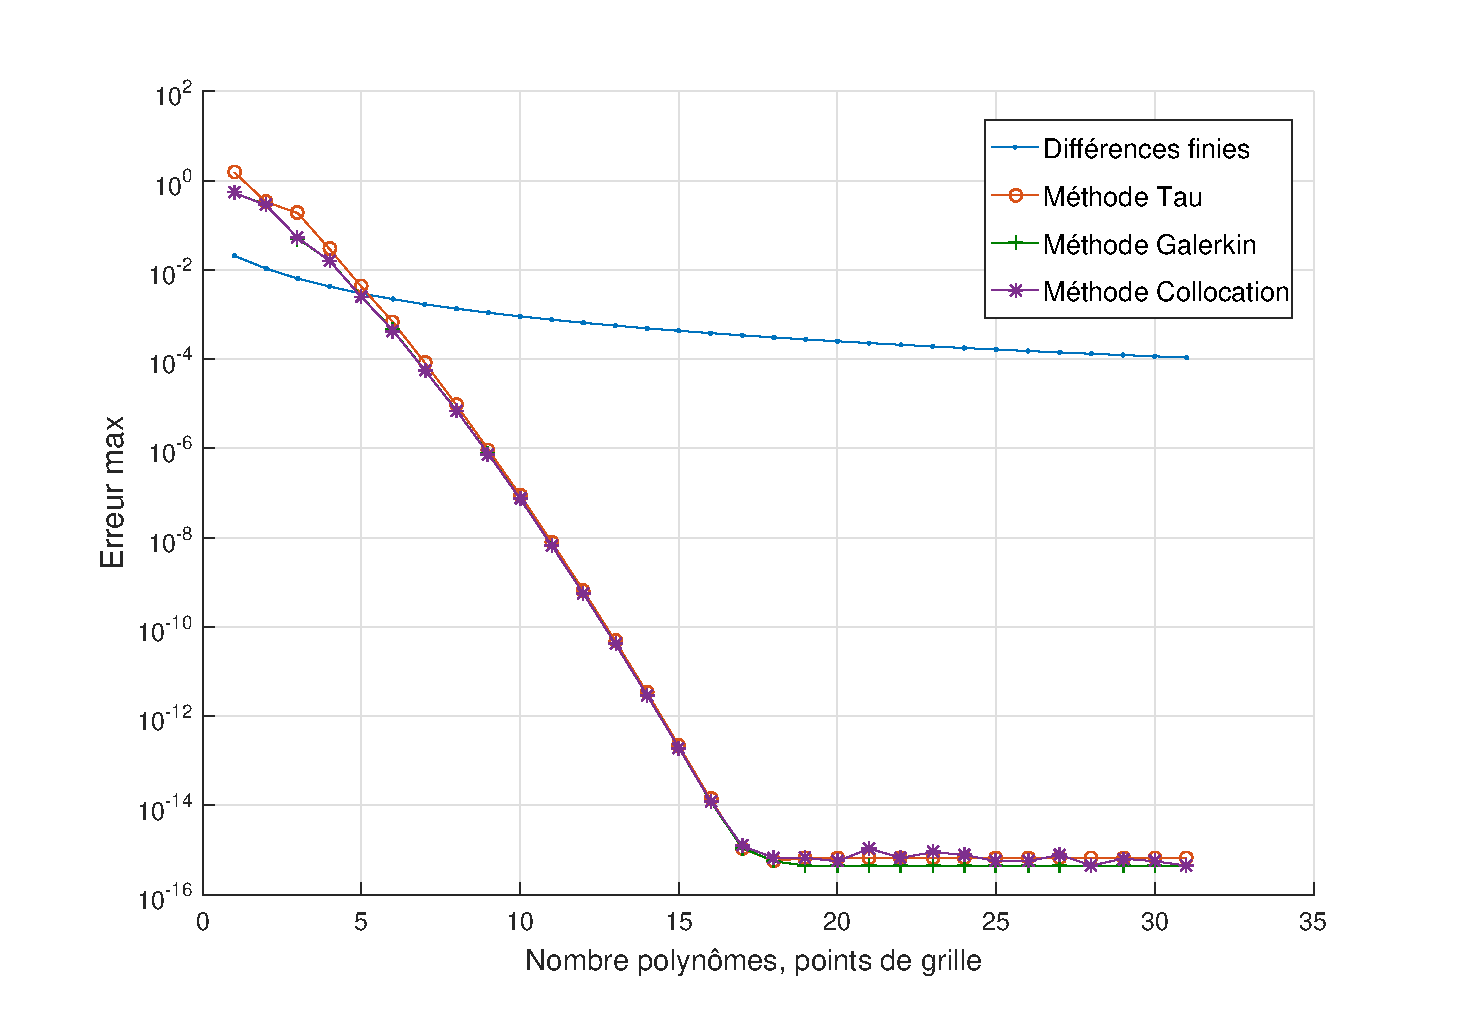
\includegraphics[width=16cm]{graphe_erreur.eps}
  \caption{Comparaison de l'erreur maximale des différentes méthodes numériques avec la solution analytique.}
  \label{fig_erreur}
\end{figure}


 \part{Exercice sur l'équation de Schrödinger}
\setcounter{section}{0}
\setcounter{equation}{0}
 
%\section{Introduction}


\section{Equation de Schrödinger stationnaire}

\subsection{Introduction}

Dans les unités atomiques ($u.a.$), l'équation de Schrödinger stationnaire à une dimension s'écrit :

\begin{equation}\label{eq:sta}
\left[\frac{1}{2}p^{2}+V(x)\right]\ket{\phi(x)}= E\ket{\phi(x)}\;,
\end{equation}

où $m_{e}=\hbar=\left|e\right|=\frac{1}{4\pi\epsilon_{0}}=1$.

On remplace le carré de l'opérateur impulsion par $p^{2}=-\frac{\partial^2}{\partial x^{2}}$ et on utilise le potentiel suivant :

\begin{equation}
V(x)= -V_{0}e^{-\alpha x^{2}}\;.
\end{equation}

Pour résoudre cette équation \eqref{eq:sta}, on utilise un développement tronqué de fonctions d'Hermite :

\begin{equation}\label{eq:varphi}
\phi(x)= \sum_{k=0}^N a_k \varphi_k(x)\;,
\end{equation}

où les fonctions d'Hermite :

\begin{equation}
\varphi_k(x)= c_{k} H_{k}(x)e^{-\frac{x^{2}}{2}}\;,
\end{equation}

avec $c_{k} =\left(2^{k}k!\sqrt{\pi}\right)^{-1/2}$ et les polynômes d'Hermite $H_{k}(x)$ , forment une base complète. Le choix des fonctions de base utilisées a été guidé par la physique du problème traité.

On a les propriétés suivantes, relation d'orthogonalité des fonctions d'Hermite :

\begin{equation}\label{eq:ortho_phi}
\int_{-\infty}^{+\infty} \varphi_m(x) \varphi_n(x) dx = \delta_{mn}\;,
\end{equation}

et les relations de récurrence des polynômes d'Hermite :

\begin{eqnarray}\label{eq:recu}
H_{k+1}(x) &=& 2xH_k(x) - 2kH_{k-1}(x) \;,\\
H'_{k}(x) &=& 2k H_{k-1}(x)\;,\label{eq:recu2}
\end{eqnarray}

pour $k \geq 1$, avec $H_0 (x) = 1$ et $H_1 (x) = 2x$.

\subsection{Résolution}

On applique le bra $\bra{\varphi_n(x)}$ à l'équation \eqref{eq:sta}. On a :

\begin{eqnarray}
\bra{\varphi_n(x)}\left[\frac{1}{2}p^{2}+V(x)\right]\ket{\phi(x)} &=& \bra{\varphi_n(x)}E\ket{\phi(x)}\;,\\
 &=& E \sum_{k=0}^N a_k \int_{-\infty}^{+\infty} \varphi_n(x)\varphi_k(x) dx\;,\\
&=& E \sum_{k=0}^N a_k \delta_{nk}\;,\\
&=& E a_n\;.
\end{eqnarray} 

On traite ensuite le membre de gauche en deux parties.

\subsubsection{Terme énergie cinétique}

\begin{equation}\label{eq:ciné}
\bra{\varphi_n(x)} \frac{1}{2}p^{2} \ket{\phi(x)} = - \frac{1}{2}\sum_{k=0}^N a_k \int_{-\infty}^{+\infty} \varphi_n(x) \frac{\partial^2}{\partial x^{2}} \varphi_k(x) dx\;,
\end{equation}

avec 

\begin{equation}
 \frac{\partial^2}{\partial x^{2}} \varphi_k(x) = \frac{1}{2}\sqrt{k(k-1)}\varphi_{k-2}(x) -\left(k+\frac{1}{2}\right)\varphi_k(x) + \frac{1}{2} \sqrt{(k+1)(k+2)}\varphi_{k+2}(x)\;,
\end{equation}

pour $k \geq 2$. On a obtenu cette forme à l'aide des relations de récurrence \eqref{eq:recu} et \eqref{eq:recu2}. En tenant compte de la relation d'orthogonalité \eqref{eq:ortho_phi}, \eqref{eq:ciné} devient :

\begin{eqnarray}
- \frac{1}{2}\sum_{k=0}^N a_k \left(\frac{1}{2}\sqrt{k(k-1)}\delta_{n,k-2} - \left(k+\frac{1}{2}\right)\delta_{nk}+ \frac{1}{2} \sqrt{(k+1)(k+2)}\delta_{n,k+2} \right) \\
= - \frac{1}{2}\left(\frac{1}{2}\sqrt{(n+1)(n+2)}a_{n+2}-\left(n+\frac{1}{2}\right)a_{n}+\frac{1}{2}\sqrt{n(n-1)}a_{n-2} \right)\;.
\end{eqnarray}

pour $n \geq 2$. Pour $n = 0,1$, on omet le dernier terme de cette expression.

\subsubsection{Terme énergie potentiel}

\begin{equation}
\bra{\varphi_n(x)} V(x)\ket{\phi(x)} = \sum_{k=0}^N a_k\int_{-\infty}^{+\infty} \varphi_n(x) V(x) \varphi_k(x) dx\;.
\end{equation}

Il n'est pas possible de trouver une solution analytique à cette intégrale. Nous allons donc utiliser la quadrature de Gauss-Hermite comme approximation.

\subparagraph{Quadrature de Gauss-Hermite.}

La quadrature de Gauss-Hermite permet d'approximer l'intégrale de la forme suivante :

\begin{equation}\label{exp_qua}
\int_{-\infty}^{+\infty} f(x) e^{-x^{2}} dx\;.
\end{equation}

Dans ce cas :

\begin{eqnarray}
\int_{-\infty}^{+\infty} f(x) e^{-x^{2}} dx & = & \sum_{i=1}^N w_i f(x_i)+C_{N}f^{(2N)}(\xi) \;,\\
& \approx & \sum_{i=1}^N w_i f(x_i)\;,
\end{eqnarray}

où $N$ est le nombre de points d'échantillonnage utilisé, $x_i$ sont les racines des polynômes d'Hermite et $w_i$ sont les poids associés.

\subparagraph{Expression de l'intégrale du terme énergie potentiel.}

On a donc :

\begin{eqnarray}
\lefteqn{\int_{-\infty}^{+\infty} \varphi_n(x) V(x) \varphi_k(x) dx }\\
&=& - \int_{-\infty}^{+\infty} c_{n} H_{n}(x)e^{-\frac{x^{2}}{2}} V_{0}e^{-\alpha x^{2}} c_{k} H_{k}(x)e^{-\frac{x^{2}}{2}} dx\;,\\
 &=& - \int_{-\infty}^{+\infty} V_{0} c_{n} c_{k} H_{n}(x) H_{k}(x) e^{-\left(1+\alpha \right)x^{2}} dx\;,\\
 &=&  \int_{-\infty}^{+\infty} \left( - \frac{V_{0} c_{n} c_{k}}{\sqrt{1+\alpha}} H_{n}\left(\frac{u}{\sqrt{1+\alpha}}\right) H_{k}\left(\frac{u}{\sqrt{1+\alpha}}\right) \right) e^{-u^{2}} du\;.
\end{eqnarray}

On a utilisé le changement de variable $x = \frac{u}{\sqrt{1+\alpha}}$ à la dernière ligne. On retrouve une expression de la forme \eqref{exp_qua}. On résoud cette intégrale en utilisant la quadrature de Gauss-Hermite. Cela se fait aisément dans Matlab à l'aide de la fonction \texttt{hermquad.m}. Celle-ci donne les $x_i$ et les $w_i$ pour $N$ fixé. On prendra $N$ suffisamment élevé pour que $f^{(2N)}(\xi) = 0$, c'est à dire, au moins le nombre de fonctions d'Hermite, $N+1$, dans l'équation \eqref{eq:varphi}. 

\subsection{Solution sous Maltab}

Dans le potentiel, si l'on prend comme valeur $V_{0} = 3$ et $\alpha = 1$, on obtient deux états liés :

\begin{align}
\begin{cases}
E_{0} = -1.963720\;, \\
E_{1} = -0.369890\;.
\end{cases}
\end{align}

Avec notre implémentation sous Matlab, on obtient ces deux valeurs d'énergie à six décimales exactes en prenant $N \geq 50$. Si l'on prend un $\alpha$ plus petit, on peut obtenir plus d'états liés.

\section{Equation de Schrödinger dépendante du temps}

\subsection{Introduction}

Dans les unités atomiques, nous allons étudier l'équation de Schrödinger dépendante du temps à une dimension suivante :

\begin{equation}\label{eq:schdt}
\dot{\imath}\hbar\frac{\partial}{\partial t}\ket{\Psi(x,t)}=\left[\frac{1}{2}p^2+ V(x)+A(t)\cdot p\right]\ket{\Psi(x,t)}\;,
\end{equation}

avec

\begin{align}
\begin{cases}
p^{2}=-\frac{\partial^2}{\partial x^{2}}\;,\\
V(x)= -V_{0}e^{-\alpha x^{2}}\;, \\
A(t)= A_{0}f(t-t_{0})\sin(\omega (t-t_{0}))\;,
  \end{cases}
\end{align}

où l'enveloppe est définie par :
\begin{equation}
f(t-t_{0})=\cos^{2} \left(\frac{\omega (t-t_{0})}{2K}\right)\;,
\end{equation}

pour $\frac{-\pi K}{\omega}<t-t_{0}<\frac{\pi K}{\omega}$ avec $K$ entier.

La fonction d'onde solution de l'équation de Schrödinger dépendante du temps est :

\begin{equation}\label{psi_t}
\Psi(x,t)= \sum_{n=0}^N b_{n}(t)\phi_n(x) e^{-iE_{n}t}\;,
\end{equation}

où 

\begin{equation}
\phi_n(x)= \sum_{k=0}^N a_{k,n} \varphi_k(x)
\end{equation}

sont les fonctions d'onde solutions de l'équation de Schrödinger stationnaire. On a la condition initiale suivante $\Psi(x,t=t_{0})= \Psi(x,0) = \phi_{0}(x)$, c'est-à-dire, l'état du fondamental.

On a la relation d'orthogonalité des fonctions d'onde solutions de l'équation de Schrödinger stationnaire :

\begin{equation}\label{eq:ortho_phin}
\int_{-\infty}^{+\infty} \phi_m(x) \phi_n(x) dx = \delta_{mn}\;.
\end{equation}

\subsection{Résolution}

On injecte \eqref{psi_t} dans \eqref{eq:schdt}, on obtient :

\begin{equation}
\sum_{n=0}^{N}\phi_{n}(x)\dot{b}_{n}(t) e^{-iE_{n}t} = - A(t) \sum_{n=0}^{N}\frac{\partial \phi_{n}(x)}{\partial x}b_{n}(t) e^{-iE_{n}t}\;.
\end{equation}

On applique le bra $\bra{\phi_{m}(x)} e^{iE_{m}t}$ à cette équation et avec la relation d'orthogonalité \eqref{eq:ortho_phin}, on obtient :

\begin{equation}
\dot{b}_{m}(t) = - A(t) \int \sum_{n=0}^{N}\phi_{m}^{\ast}(x)\frac{\partial \phi_{n}(x)}{\partial x}b_{n}(t) e^{-i(E_{n}-E_{m})t} dx\;.
\end{equation}

On pose :

\begin{equation}
I_{m,n}= \int \phi_{m}^{\ast}(x)\frac{\partial \phi_{n}(x)}{\partial x} dx\;.
\end{equation}

Pour résoudre cette intégrale, on commence par réécrire son intégrant à l'aide des fonctions d'Hermite :

\begin{equation}
\phi_{m}^{\ast}(x)\frac{\partial \phi_{n}(x)}{\partial x} = \sum_{k=0}^{N} a_{k,m}^{\ast}\varphi_{k}^{\ast} \cdot \left(\sum_{l=1}^{N}a_{l,n} \sqrt{\frac{l}{2}}\varphi_{l-1}(x)-\sum_{l=0}^{N-1}a_{l,n}\sqrt{\frac{l+1}{2}}\varphi_{l+1} \right)\;,
\end{equation}

où on a pris :

\begin{equation}
\varphi'_{l}(x) =  \sqrt{\frac{l}{2}} \varphi_{l-1}(x)-\sqrt{\frac{l+1}{2}}\varphi_{l+1}(x)\;.
\end{equation}

Après intégration, avec la relation d'orthogonalité des fonctions d'Hermite \eqref{eq:ortho_phi}, en posant $l=k+1$ dans le premier terme de la parenthèse et $l=k-1$ dans le second :

\begin{equation}
I_{m,n} = \sum_{k=0}^{N-1} a_{k,m}^{\ast}  a_{k+1,n} \sqrt{\frac{k+1}{2}}- \sum_{k=1}^{N} a_{k,m}^{\ast}a_{k-1,n}\sqrt{\frac{k}{2}}\;,
\end{equation}

pour $m,n = 0,1,..,N$. Où l'on peut remarquer que la première somme termine à $N-1$ et la seconde commence à $1$, car $0 \leq k \leq N$ doit être respecté.

On a donc finalement :

\begin{equation}
\dot{b}_{m}(t) = - A(t) \sum_{n=0}^{N}I_{m,n}b_{n}(t) e^{-i(E_{n}-E_{m})t}\;,
\end{equation}
pour $m=0,...,N$.

\subsection{Solution sous Matlab}

On implémente cette fonction dans Matlab avec \texttt{Ode15s} pour trouver les $b(t)$. On aura sous forme matricielle :

\begin{equation}
\frac{d}{dt}
\begin{pmatrix}
 b_{0}\\ 
 b_{1}\\ 
 \vdots\\ 
 b_{N-1}\\ 
  b_{N}
\end{pmatrix} = -A(t) \cdot M(t) \cdot 
\begin{pmatrix}
 b_{0}\\ 
 b_{1}\\ 
 \vdots\\ 
 b_{N-1}\\ 
  b_{N}
\end{pmatrix}\;,
\end{equation}

où $M(t)$ est le produit d'Hadamard (commande Matlab: \texttt{.*}) des matrices $I_{m,n}$ et $e^{-i(E_{n}-E_{m})t}$. 

Pour le calcul numérique, on a pris $N=80$. Sur un de nos ordinateurs personnels équipé d'un processeur <<Intel Q6600>>, notre routine Matlab, avec $N=80$, tourne environ 40 minutes pour afficher un graphique. 

De plus, on reprend les mêmes valeurs pour le potentiel : $V_{0} = 3$ et $\alpha = 1$. Pour le potentiel vecteur $A(t)$, on prendra $t_{0}=0$. On choisira différents $\omega$, $K$ et $A_{0}$.

On prend les conditions initiales : $b_{0}=1$ et $b_{n}=0$ pour $n > 0$, c'est-à-dire que l'état initial est dans le fondamental.

On représente graphiquement (figures 3 à 11), les probabilités d'être dans le fondamental, dans le second état lié ou d'être ionisé, en fonction du temps $t$ : 

\begin{equation}
\mathcal{P}_{0}=\left| b_{0}(t)\right|^2= b^\ast_0(t)b_0(t)\;,
\end{equation}

\begin{equation}
\mathcal{P}_{1}=\left| b_{1}(t)\right|^2= b^\ast_1(t)b_1(t)\;,
\end{equation}

\begin{equation}
\mathcal{P}_{I}=1-\left| b_{0}(t)\right|^2-\left| b_{1}(t)\right|^2\;.
\end{equation}

On obtient la formule de la probabilité d'ionisation à partir de :

\begin{equation}
\sum_{n=0}^{N} \left| b_{n}(t)\right|^2 =1\;.
\end{equation}


Lorsque l'on est à la résonance :

\begin{eqnarray}
\omega_{r} &=& E_{1}-E_{0}\;,\\
&\approx& 1.59383\;.
\end{eqnarray}

\subsubsection{Répartition des niveaux d'énergie}

Sur la figure \ref{fig_repartition_energie}, on a représenté les 81 niveaux d'énergie, issu de l'équation de Schrödinger stationnaire, lorsqu'on prend $N=80$ dans le développement tronqué de fonctions d'Hermite (équation \eqref{eq:varphi}). On y a ajouté le potentiel utilisé ($V(x)= -3e^{- x^{2}}$).

On observe bien les deux états liés croisant le potentiel. De plus, on s'aperçoit que dans le continuum ($E>0$), la densité des états est plus élevée proche de zéro et diminue au fur et à mesure qu'on s'en éloigne.

\subsubsection{Observations sur les graphiques des probabilités}

\paragraph{Résonance}

A la fréquence de résonance, $\omega = \omega_{r}$, on observe (figures \ref{fig_N80_K20_A1}, \ref{fig_N80_K30_A1} et \ref{fig_N80_K20_A4}) que les courbes des probabilités d'occupation des deux états liés oscillent en opposition de phase. Ce sont les oscillations de Rabi.

En outre, on observe sur les graphiques à la résonance (figures \ref{fig_N80_K20_A1} et \ref{fig_N80_K30_A1}) que les derniers pics des probabilités d'être dans les états liés sont plus élevés que leur précédent. Alors que l'amortissement devrait se poursuive. Cela est sans doute dû au faible nombre de fonctions de base utilisées ($N=80$). La densité des états dans la région du continuum où le système arrive après avoir absorbé deux photons ($E \approx 1.22394$) n'est pas suffisante.

\paragraph{Autres fréquences}

Pour $\omega = 0.8$ (figure \ref{fig_N80_W08_K30_A1}) et $\omega = 3.2$ (figure \ref{fig_N80_W32_K30_A1}), on constate que le transfert de population entre les deux états liés est plus faible que pour $\omega = \omega_{r}$ (figure \ref{fig_N80_K30_A1}). Car nous ne sommes pas à la résonance.

D'autre part, pour $\omega = 2$ (figure \ref{fig_N80_W2_K20_A1}) et $\omega = 3.2$ (figure \ref{fig_N80_W32_K30_A1} et \ref{fig_N80_W32_K40_A1}), l'amortissement est régulier. Il n'y a pas de chute de la probabilité d'ionisation comme sur les graphiques pour $\omega = \omega_{r}$ (figures \ref{fig_N80_K20_A1} et \ref{fig_N80_K30_A1}). La qualité de ces graphes peut être dû à la densité d'états élevée dans la zone du continuum pour $\omega = 2$ après absorption d'un photon mais cet argument ne tient plus pour $\omega = 3.2$.

\paragraph{Probabilité d'ionisation}

On peut observer sur les graphiques des $\omega = \omega_{r}$ (figures \ref{fig_N80_K20_A1} et \ref{fig_N80_K30_A1}), $\omega = 0.8$ (figures \ref{fig_N80_W08_K10_A1} et \ref{fig_N80_W08_K30_A1}) et $\omega = 3.2$ (figures \ref{fig_N80_W32_K30_A1} et \ref{fig_N80_W32_K40_A1}), ayant respectivement des $K$ différents et le reste des valeurs identique, que la probabilité d'ionisation, $\mathcal{P}_{I}$, augmente avec $K$ et donc avec la durée de l'impulsion ($t_{max}= \frac{\pi K}{\omega}$).

Par ailleurs, pour un temps d'impulsion donné, la probabilité d'ionisation est maximale à la résonance. Sur un graphe de $\mathcal{P}_{I}$ en fonction de $\omega$, elle forme un pic à la résonance. Sur nos graphiques (figures \ref{fig_N80_K20_A1}, \ref{fig_N80_W08_K10_A1} et \ref{fig_N80_W32_K40_A1}) à durée d'impulsion identique ($t_{max} \approx 40\ u.a.$) et $\omega$ différents, on a bien que $\mathcal{P}_{I}$ est maximale à la résonance. 

Finalement, nous pouvons observer que la probabilité d'ionisation dépend de l'intensité du signal, c'est à dire de $A(t)^2$. Sur les graphiques à la résonance avec $K=20$ (figures \ref{fig_N80_K20_A1} et \ref{fig_N80_K20_A4}), ainsi que sur ceux avec $\omega = 3.2$ et $K=30$ (figures \ref{fig_N80_W32_K30_A1}, \ref{fig_N80_W32_K30_A4}), on observe l'augmentation de $\mathcal{P}_{I}$ avec $A_0$. On voit que $\mathcal{P}_{I}$ se rapproche de 1 lorsque $A_0$ augmente.

\begin{figure}[p]
\begin{center}
  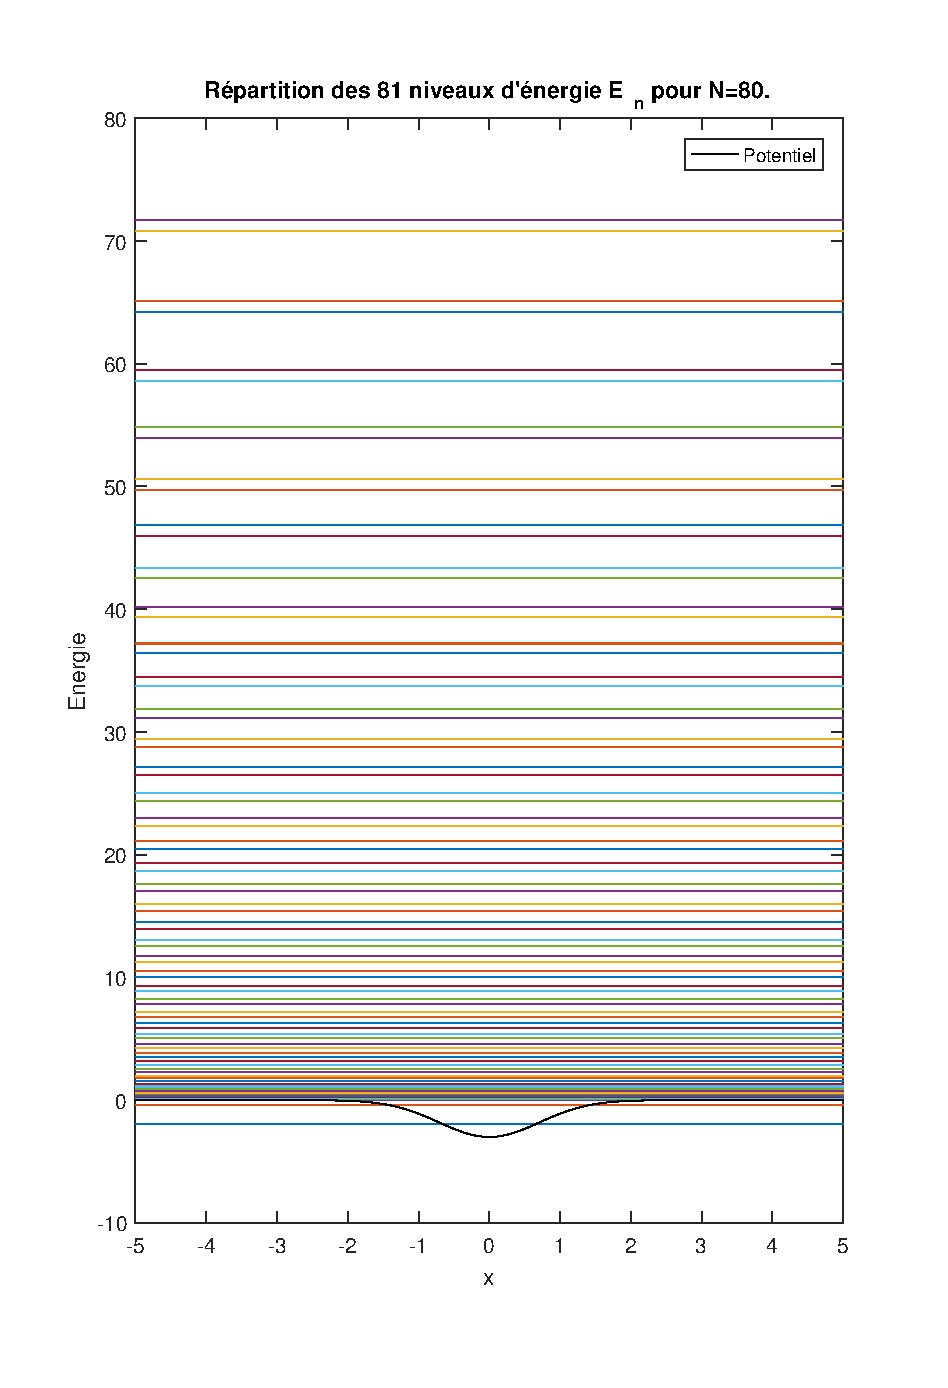
\includegraphics[height=18cm]{repartition_energie.eps}
  \end{center}
  \caption{}
  \label{fig_repartition_energie}
\end{figure}

\begin{figure}
	\begin{center}
  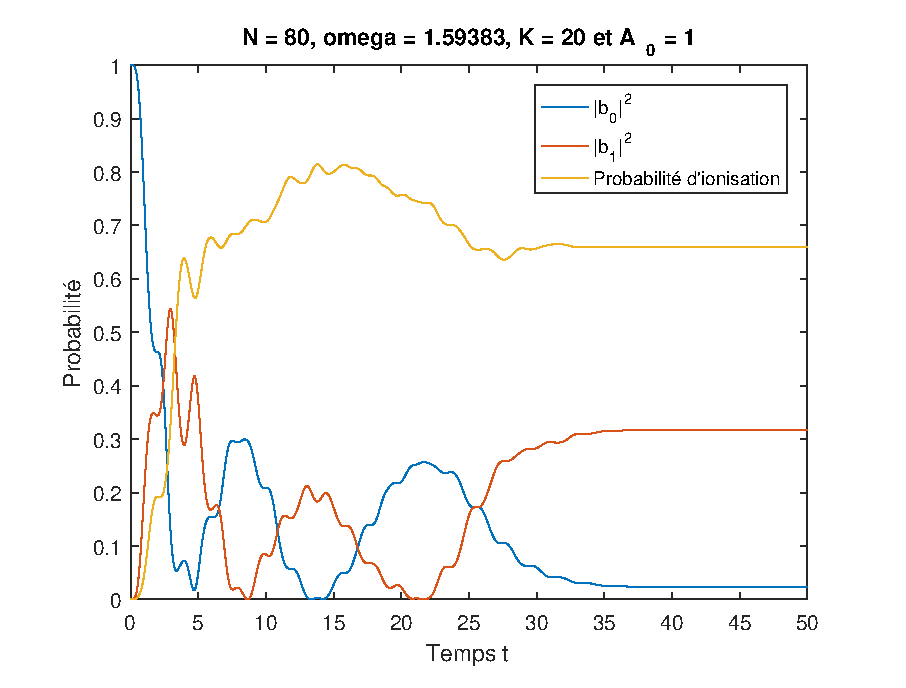
\includegraphics[height=8.3cm]{N80_K20_A1.eps}
    \end{center}
  \caption{}
  \label{fig_N80_K20_A1}
\end{figure}


\begin{figure}
\begin{center}
  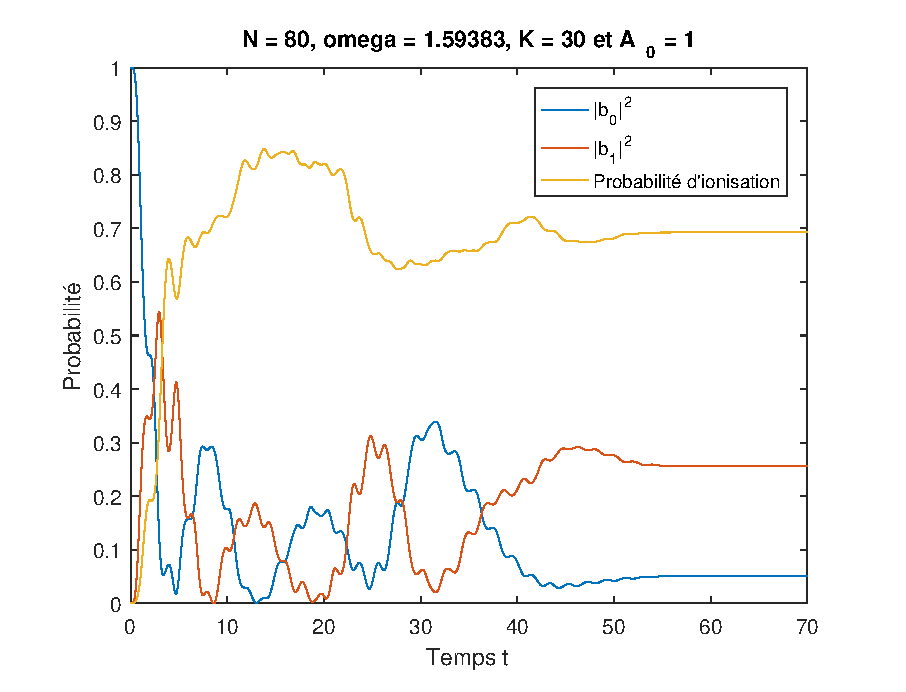
\includegraphics[height=8.3cm]{N80_K30_A1.eps}
      \end{center}
  \caption{}
  \label{fig_N80_K30_A1}
\end{figure}

\begin{figure}
\begin{center}
  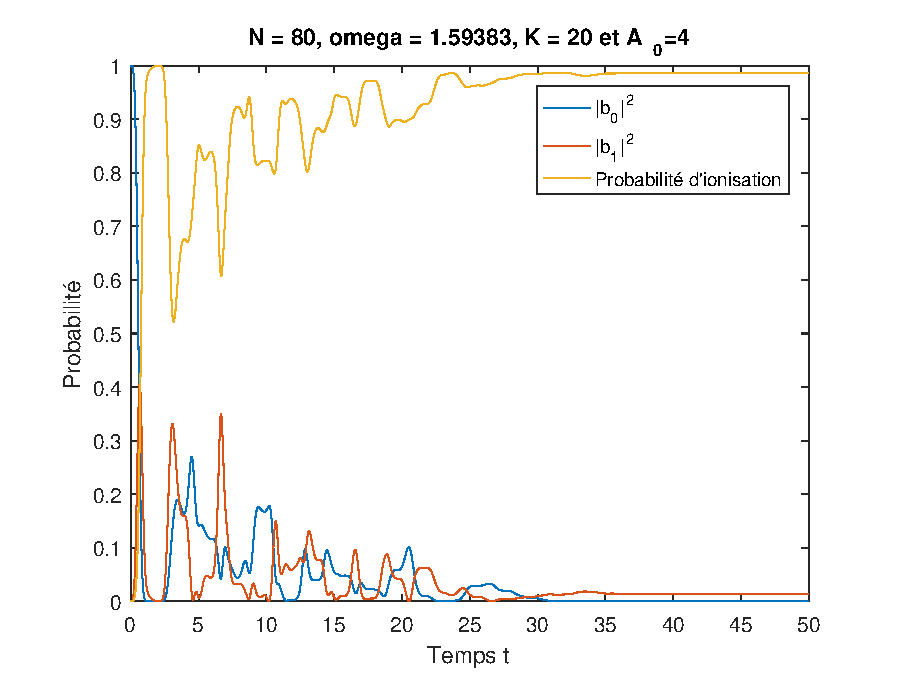
\includegraphics[height=8.3cm]{N80_K20_A4.eps}
      \end{center}
  \caption{}
  \label{fig_N80_K20_A4}
\end{figure}

\begin{figure}
\begin{center}
  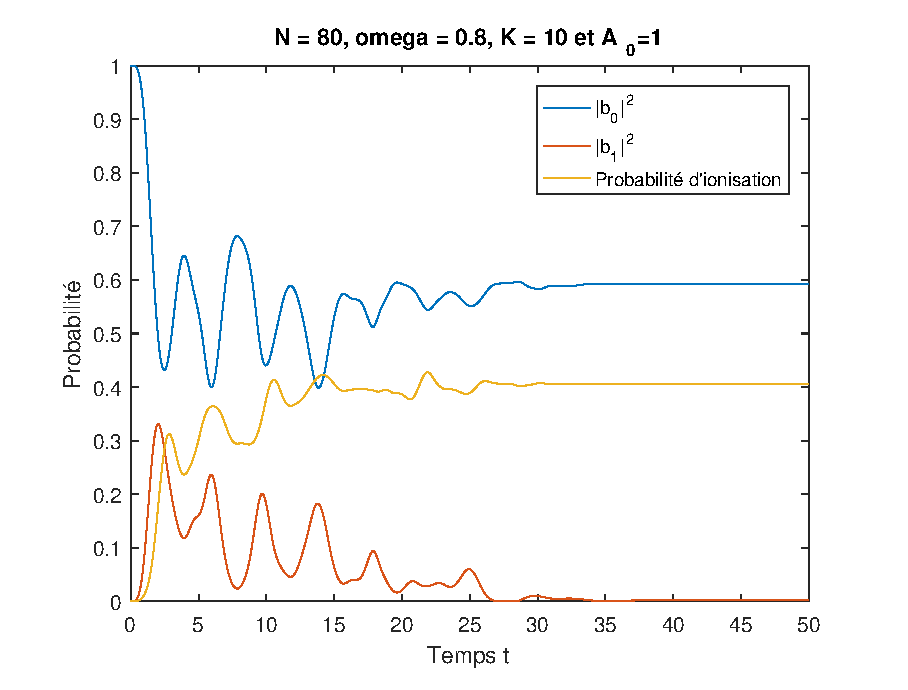
\includegraphics[height=8.3cm]{N80_W08_K10_A1.eps}
      \end{center}
  \caption{}
  \label{fig_N80_W08_K10_A1}
\end{figure}

\begin{figure}
\begin{center}
  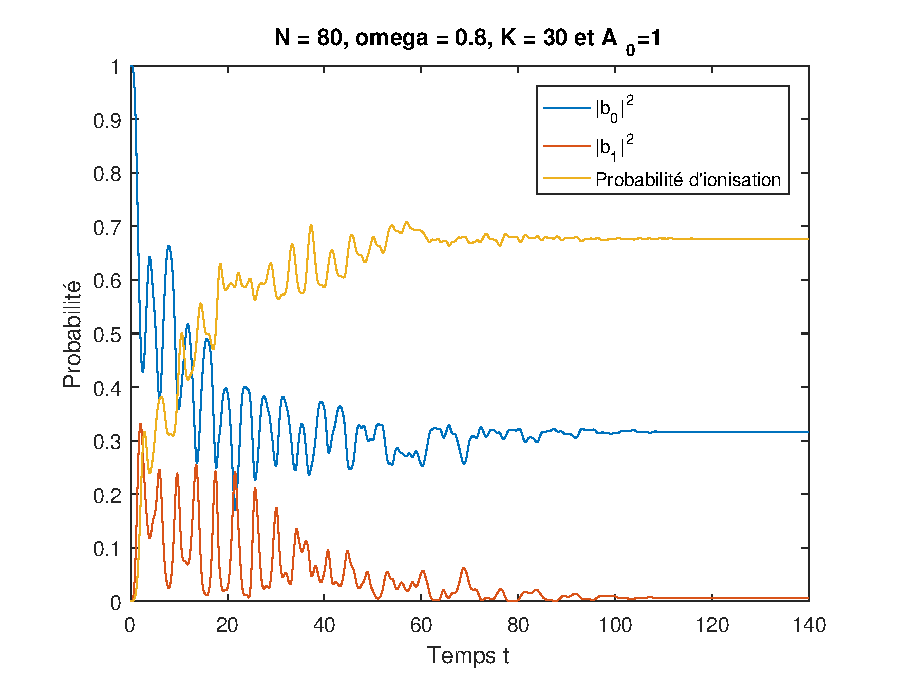
\includegraphics[height=8.3cm]{N80_W08_K30_A1.eps}
      \end{center}
  \caption{}
  \label{fig_N80_W08_K30_A1}
\end{figure}

\begin{figure}
\begin{center}
  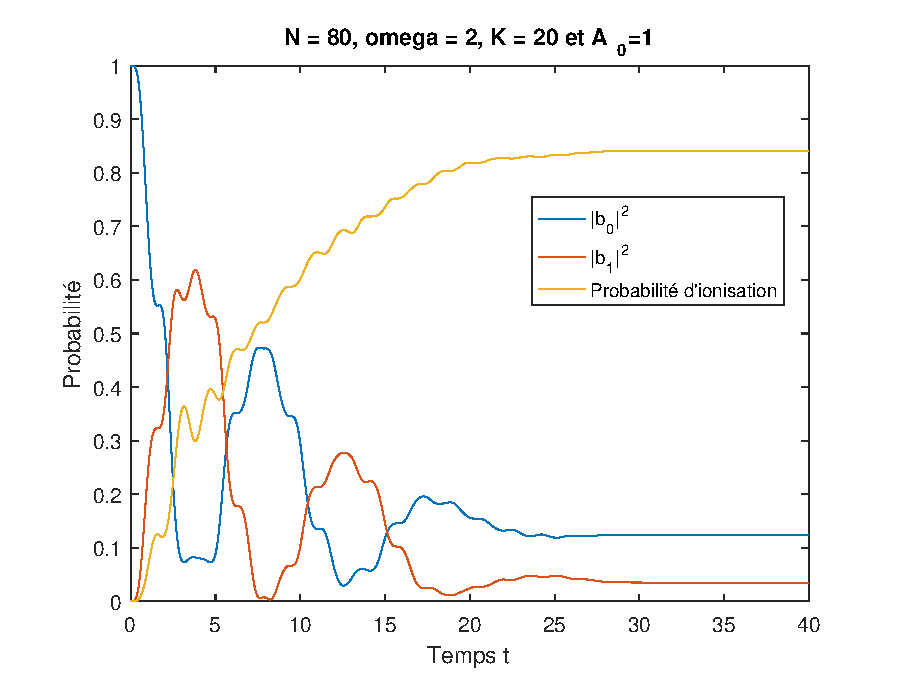
\includegraphics[height=8.3cm]{N80_W2_K20_A1.eps}
      \end{center}
  \caption{}
  \label{fig_N80_W2_K20_A1}
\end{figure}

\begin{figure}
\begin{center}
  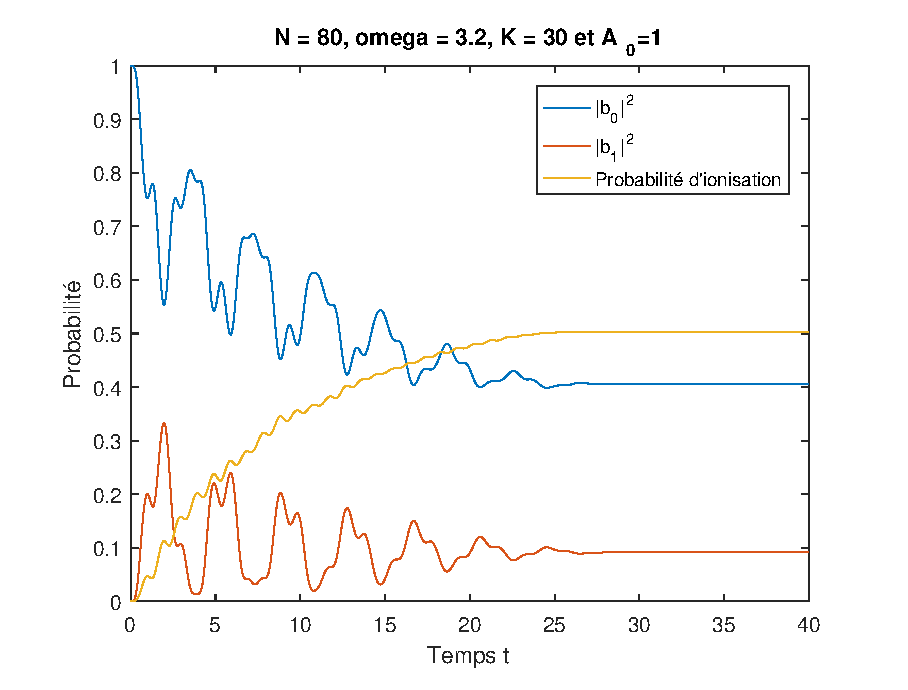
\includegraphics[height=8.3cm]{N80_W32_K30_A1.eps}
      \end{center}
  \caption{}
  \label{fig_N80_W32_K30_A1}
\end{figure}

\begin{figure}
\begin{center}
  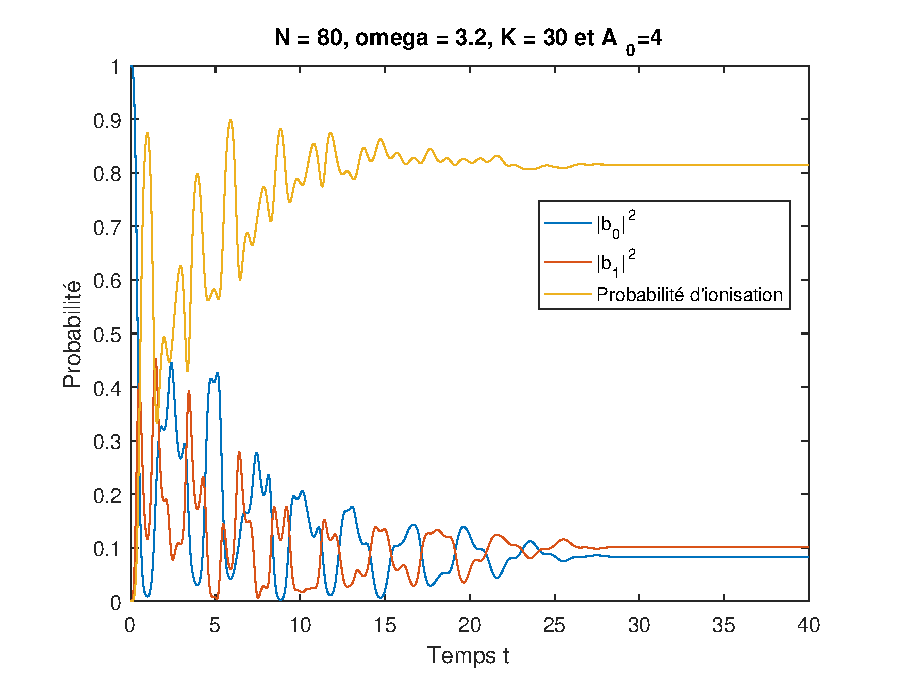
\includegraphics[height=8.3cm]{N80_W32_K30_A4.eps}
      \end{center}
  \caption{}
  \label{fig_N80_W32_K30_A4}
\end{figure}

\begin{figure}
\begin{center}
  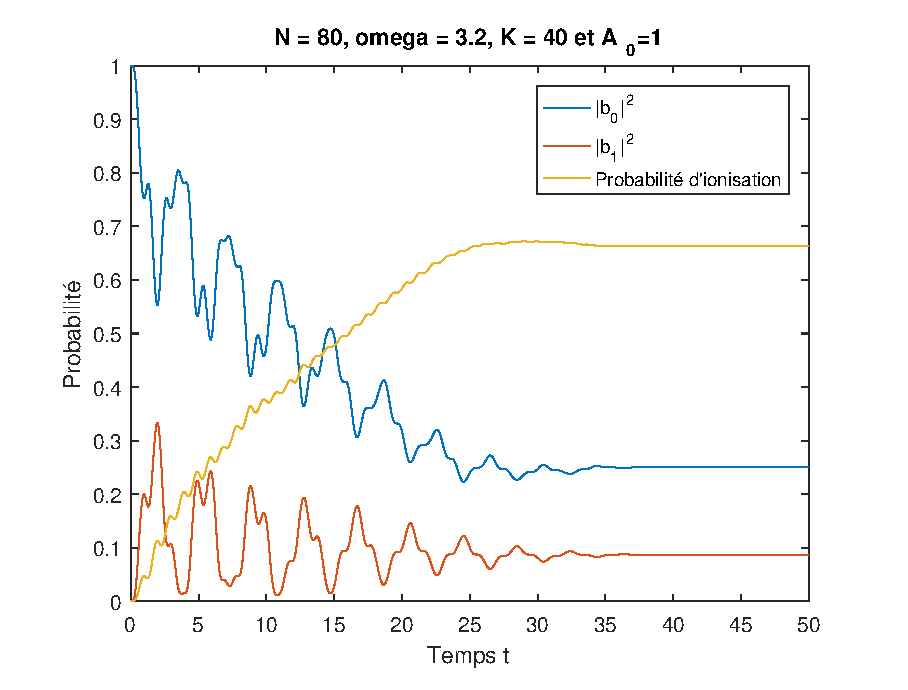
\includegraphics[height=8.3cm]{N80_W32_K40_A1.eps}
      \end{center}
  \caption{}
  \label{fig_N80_W32_K40_A1}
\end{figure}

\end{document}
